\ifdefined\maindoc
\appendix
\else
% typesetting this chapter as a standalone document
\def\doctitle{Mathematical Review}
% starting definitions for both the main document and stand-alone chapters
\documentclass{book}

\def\mech{artisynth.core.mechmodels}
\def\mgeo{maspack.geometry}

% Add search paths for input files
\makeatletter
\def\input@path{{../}{../../}{../texinputs/}}
\makeatother

\usepackage{amsmath}
\usepackage{framed}
%%
%% Default settings for artisynth
%%
\NeedsTeXFormat{LaTeX2e}
%%\ProvidesPackage{artisynthDoc}[2012/04/05]

\usepackage[T1]{fontenc}
\usepackage[latin1]{inputenc}
\usepackage{listings}
\usepackage{makeidx}
\usepackage{latexml}
\usepackage{graphicx}
\usepackage{framed}
\usepackage{booktabs}
\usepackage{color}

\newcommand{\pubdate}{\today}
\newcommand{\setpubdate}[1]{\renewcommand{\pubdate}{#1}}
\newcommand{\code}[1]{{\tt #1}}

\iflatexml
\usepackage{hyperref}
\setlength\parindent{0pt} 
\else
%% then we are making a PDF, so include things that LaTeXML can't handle: 
%% docbook style, \RaggedRight
\usepackage{ifxetex}
\usepackage{xstring}
\usepackage{pslatex} % fixes fonts; in particular sets a better-fitting \tt font

\usepackage[most]{tcolorbox}
\definecolor{shadecolor}{rgb}{0.95,0.95,0.95}
\tcbset{
    frame code={}
    center title,
    left=0pt,
    right=0pt,
    top=0pt,
    bottom=0pt,
    colback=shadecolor,
    colframe=white,
    width=\dimexpr\textwidth\relax,
    enlarge left by=0mm,
    boxsep=0pt,
    arc=0pt,outer arc=0pt,
}%

\usepackage[A4]{artisynth_papersize}
%\usepackage[letter]{artisynth_papersize}
\usepackage[hyperlink]{asciidoc-dblatex} 

%\usepackage{verbatim}
\usepackage{ragged2e}
\setlength{\RaggedRightRightskip}{0pt plus 4em}
\RaggedRight
\renewcommand{\DBKpubdate}{\pubdate}
\renewcommand{\DBKreleaseinfo}{}
\fi

% set hypertext links to be dark blue:
\definecolor{darkblue}{rgb}{0,0,0.8}
\definecolor{sidebar}{rgb}{0.5,0.5,0.7}
\hypersetup{colorlinks=true,urlcolor=darkblue,linkcolor=darkblue,breaklinks=true}

%%%%%%%%%%%%%%%%%%%%%%%%%%%%%%%%%%%%%%%%%%%%%%%%%%%%%%%%%%%%%%%%%%%%%%%%%%%%%
%
% Define macros for handling javadoc class and method references
%
%%%%%%%%%%%%%%%%%%%%%%%%%%%%%%%%%%%%%%%%%%%%%%%%%%%%%%%%%%%%%%%%%%%%%%%%%%%%%
\makeatletter

% macro to enable line break if inside a PDF file
\def\pdfbreak{\iflatexml\else\\\fi}

% code inspired by http://stackoverflow.com/questions/2457780/latex-apply-an-operation-to-every-character-in-a-string
\def\removeargs #1{\doremoveargs#1$\wholeString\unskip}
\def\doremoveargs#1#2\wholeString{\if#1$%
\else\if#1({()}\else{#1}\taketherest#2\fi\fi}
\def\taketherest#1\fi
{\fi \doremoveargs#1\wholeString}

% Note: still doesn't work properly when called on macro output ...
% i.e., \dottoslash{\concatnames{model}{base}{foo}} fails 
\def\dottoslash #1{\dodottoslash#1$\wholeString\unskip}
\def\dodottoslash#1#2\wholeString{\if#1$%
\else\if#1.{/}\else{#1}\fi\dottaketherest#2\fi}
\def\dottaketherest#1\fi{\fi \dodottoslash#1\wholeString}

\def\hashtodot #1{\dohashtodot#1$\wholeString\unskip}
\def\dohashtodot#1#2\wholeString{\if#1$X%
\else\if#1\#{.}\else{#1}\fi\hashtaketherest#2\fi}
\def\hashtaketherest#1\fi{\fi \dohashtodot#1\wholeString}

%\dollartodot{#1} does the same thing as \StrSubstitute[0]{#1}{\$}{.}
% from the packahe xstring. We define \dollartodot instead because
% LaTeXML does not implement xstring.
%
% Note that for the substituion to work, we need \ifx instead of \if,
% since otherwise escaped characters won't work properly:
% if #1 = \$, then \if#1* seems to compare '\' and '$' (and output '*'),
% rather than comparing '$' to '*'
\def\dollartodot #1{\dodollartodot#1*\wholeString\unskip}
\def\dodollartodot#1#2\wholeString{\ifx#1*%
\else \ifx#1\${.}\else{#1}\fi\dollartaketherest#2\fi}
\def\dollartaketherest#1\fi{\fi \dodollartodot#1\wholeString}

% concatenates up to three class/method names together, adding '.' characters
% between them. The first and/or second argument may be empty, in which case
% the '.' is omitted. To check to see if these arguments are empty, we
% use a contruction '\if#1@@', which will return true iff #1 is empty
% (on the assumption that #1 will not contain a '@' character).
\def\concatnames
#1#2#3{\if#1@@\if#2@@#3\else #2.#3\fi\else\if#2@@#1.#3\else#1.#2.#3\fi\fi}

\newcommand{\javabase}{}
\newcommand{\setjavabase}[1]{\renewcommand{\javabase}{#1}}

\def\artisynthDocBase{@ARTISYNTHDOCBASE}

\iflatexml
\def\ifempty#1{\def\temp{#1}\ifx\temp\empty}%
\newcommand{\artisynthManual}[3][]{%
   \ifempty{#1}
      \href{@ARTISYNTHDOCBASE/#2/#2.html}{#3}%
    \else
      \href{@ARTISYNTHDOCBASE/#1/#2.html}{#3}%
    \fi
}
\else
\newcommand{\artisynthManual}[3][]{%
\href{https://www.artisynth.org/@ARTISYNTHDOCBASE/#2.pdf}{#3}}
\fi

%\href{@ARTISYNTHDOCBASE/#2/#2.html}{#3}}



\newcommand{\javaclassx}[2][]{%
% Includes code to prevent an extra '.' at the front if #1 is empty. It
% works like this: if '#1' is empty, then '#1.' expands to '.', and so 
% '\if#1..' will return true, in which case we just output '#2'.
\href{@JDOCBEGIN/\concatnames{\javabase}{#1}{#2}@JDOCEND}{#2}}
\newcommand{\javaclass}[2][]{%
\href{@JDOCBEGIN/\concatnames{}{#1}{#2}@JDOCEND}{\dollartodot{#2}}}
\newcommand{\javaclassAlt}[2]{%
\href{@JDOCBEGIN/\concatnames{}{}{#1}@JDOCEND}{#2}}

\newcommand{\javamethodArgsx}[2][]{%
\href{@JDOCBEGIN/\concatnames{\javabase}{#1}{#2}@JDOCEND}{#2}}
\newcommand{\javamethodArgs}[2][]{%
\href{@JDOCBEGIN/\concatnames{}{#1}{#2}@JDOCEND}{#2}}
\newcommand{\javamethodAlt}[2]{%
\href{@JDOCBEGIN/\concatnames{}{}{#1}@JDOCEND}{#2}}
\newcommand{\javamethodAltx}[2]{%
\href{@JDOCBEGIN/\concatnames{\javabase}{}{#1}@JDOCEND}{#2}}

\newcommand{\javamethodNoArgsx}[2][]{%
\href{@JDOCBEGIN/\concatnames{\javabase}{#1}{#2}@JDOCEND}{\removeargs{#2}}}
\newcommand{\javamethodNoArgs}[2][]{%
\href{@JDOCBEGIN/\concatnames{}{#1}{#2}@JDOCEND}{\removeargs{#2}}}

\newcommand{\javamethod}{\@ifstar\javamethodNoArgs\javamethodArgs}
\newcommand{\javamethodx}{\@ifstar\javamethodNoArgsx\javamethodArgsx}

%%%%%%%%%%%%%%%%%%%%%%%%%%%%%%%%%%%%%%%%%%%%%%%%%%%%%%%%%%%%%%%%%%%%%%%%%%%%%
%
% Define macros for sidebars
%
%%%%%%%%%%%%%%%%%%%%%%%%%%%%%%%%%%%%%%%%%%%%%%%%%%%%%%%%%%%%%%%%%%%%%%%%%%%%%

\iflatexml
\newenvironment{sideblock}{\begin{quote}}{\end{quote}}
\else
\usepackage[strict]{changepage}
\definecolor{sidebarshade}{rgb}{1.0,0.97,0.8}
\newenvironment{sideblock}{%
    \def\FrameCommand{%
    \hspace{1pt}%
    {\color{sidebar}\vrule width 2pt}%
    %{\vrule width 2pt}%
    {\color{sidebarshade}\vrule width 4pt}%
    \colorbox{sidebarshade}%
  }%
  \MakeFramed{\advance\hsize-\width\FrameRestore}%
  \noindent\hspace{-4.55pt}% disable indenting first paragraph
  \begin{adjustwidth}{}{7pt}%
  %\vspace{2pt}\vspace{2pt}%
}
{%
  \vspace{2pt}\end{adjustwidth}\endMakeFramed%
}
\fi

\iflatexml
\newenvironment{shadedregion}{%
  \definecolor{shadecolor}{rgb}{0.96,0.96,0.98}%
  \begin{shaded*}%
% Put text inside a quote to create a surrounding blockquote that
% will properly accept the color and padding attributes
  \begin{quote}%
}
{%
  \end{quote}%
  \end{shaded*}%
}
\else
\newenvironment{shadedregion}{%
  \definecolor{shadecolor}{rgb}{0.96,0.96,0.98}%
  \begin{shaded*}%
}
{%
  \end{shaded*}%
}
\fi

% Wanted to create a 'listing' environment because lstlisting is
% tedious to type and because under latexml it may need
% some massaging to get it to work properly. But hard to do
% because of the verbatim nature of listing
%\iflatexml
%\newenvironment{listing}{\begin{lstlisting}}{\end{lstlisting}}%
%\else
%\newenvironment{listing}{\begin{lstlisting}}{\end{lstlisting}}%
%\fi

\iflatexml\else
% fancyhdr was complaining that it wanted a 36pt header height ...
\setlength{\headheight}{36pt}
\fi

% macro for backslash character
\newcommand\BKS{\textbackslash}

% macro for double hyphen (to prevent conversion of -- into -)
\newcommand\DHY{-{}-}

% Convenience stuff
\newcommand{\ifLaTeXMLelse}[2]{%
  \iflatexml %
  #1 %
  \else %
  #2 %
  \fi %
}

\newcommand{\ifLaTeXML}[1]{ %
  \iflatexml %
  #1 %
  \fi %
}

% new methodtable environment for documenting methods

% base width of the method table
\newlength{\methodtablewidth}
\iflatexml
\setlength{\methodtablewidth}{1.6\textwidth}
\else
\setlength{\methodtablewidth}{0.94\textwidth}
\fi
% horizontal space added at end of call to \methodentry
\newlength{\methodskip}
\setlength{\methodskip}{0pt}
% lengths set inside methodtable environment:
\newlength{\methodsiglength} % length of the method signature
\newlength{\methodcomlength} % length of the method comment
\setlength{\methodsiglength}{0.5\methodtablewidth}
\setlength{\methodcomlength}{0.5\methodtablewidth}

% command to add a method to a method table:
% arg #1: package and signature for finding URL
% arg #2: anchor text
% arg #3: comment describing the method
\newcommand{\methodentry}[3]{%
\javamethodAlt{#1}{\parbox[t]{\methodsiglength}{#2}}&
{\parbox[t]{\methodcomlength}{#3}}\\%
\noalign{\vspace{\methodskip}}}

% methodtable environment takes two arguments, both scale factors for
% methodtablewidth:
% arg #1: width of the method signature column
% arg #2: width of the method comment column
\newenvironment{methodtable}[3][0pt]{%
\begingroup
\setlength{\topskip}{0pt}
\setlength{\methodskip}{#1}
\setlength{\methodsiglength}{#2\methodtablewidth}%
\setlength{\methodcomlength}{#3\methodtablewidth}%
\iflatexml
\begin{snugshade}
\else
\begin{tcolorbox}
\fi
\renewcommand{\arraystretch}{1}
\begin{tabular}{ll}}{%
\end{tabular}
\renewcommand{\arraystretch}{1}
\iflatexml
\end{snugshade}
\else
\end{tcolorbox}
\fi
\endgroup}

% commands for added top, mid and bottom lines in the table.
% uses booktabs for PDF, regular hline for HTML
\newcommand{\topline}{\iflatexml\hline\else\toprule\fi}
\newcommand{\midline}{\iflatexml\hline\else\midrule\fi}
\newcommand{\botline}{\iflatexml\hline\else\bottomrule\fi}
\newcommand{\blankline}{%
\multicolumn{2}{l}{\iflatexml{@SPACE}\else\phantom{M}\fi}\\}%
% add vertical space within a two colum method environment
\newcommand{\methodspace}[1]{%
\iflatexml
\multicolumn{2}{l}{@VERTSPACE[#1]}\\
\else
\noalign{\vspace{#1}}%
\fi}%
% break a line and add an indentation of 1em
\newcommand{\brh}{\\\phantom{M}}

\makeatother

\def\matl{\left(\begin{matrix}}
\def\matr{\end{matrix}\right)}

\def\Bthe{\boldsymbol\theta}
\def\Btau{\boldsymbol\tau}
\def\Bom{\boldsymbol\omega}
\def\Bdel{\boldsymbol\delta}
\def\Blam{\boldsymbol\lambda}
\def\Bphi{\boldsymbol\phi}
\def\Bxi{\boldsymbol\xi}
\def\Bgam{\boldsymbol\gamma}
\def\Bsig{\boldsymbol\sigma}
\def\Bnu{\boldsymbol\nu}
\def\Bmu{\boldsymbol\mu}

\def\A{{\bf A}}
\def\B{{\bf B}}
\def\C{{\bf C}}
\def\D{{\bf D}}
\def\F{{\bf F}}
\def\G{{\bf G}}
\def\H{{\bf H}}
\def\I{{\bf I}}
\def\J{{\bf J}}
\def\K{{\bf K}}
\def\Jc{{\bf J}_c}
\def\L{{\bf L}}
\def\M{{\bf M}}
\def\N{{\bf N}}
\def\O{{\bf O}}
\def\P{{\bf P}}
\def\Q{{\bf Q}}
\def\R{{\bf R}}
\def\T{{\bf T}}
\def\U{{\bf U}}
\def\W{{\bf W}}
\def\X{{\bf X}}
\def\Minv{{\bf M}^{-1}}

\def\a{{\bf a}}
\def\b{{\bf b}}
\def\c{{\bf c}}
\def\d{{\bf d}}
\def\e{{\bf e}}
\def\f{{\bf f}}
\def\g{{\bf g}}
\def\k{{\bf k}}
\def\l{{\bf l}}
\def\m{{\bf m}}
\def\n{{\bf n}}
\def\p{{\bf p}}
\def\q{{\bf q}}
\def\r{{\bf r}}
\def\u{{\bf u}}
\def\v{{\bf v}}
\def\w{{\bf w}}
\def\x{{\bf x}}
\def\y{{\bf y}}
\def\z{{\bf z}}

\def\ma{{\bf m}_\alpha}
\def\mb{{\bf m}_\beta}
\def\va{{\bf v}_\alpha}
\def\vb{{\bf v}_\beta}
\def\vp{{\bf v}_\rho}
\def\vk{{\bf v}_k}
\def\ua{{\bf u}_\alpha}
\def\ub{{\bf u}_\beta}
\def\uk{{\bf u}_k}
\def\uj{{\bf u}_j}
\def\mar{{\bf m}_{\alpha r}}
\def\mbr{{\bf m}_{\beta r}}

\def\Maa{{\bf M}_{\alpha\alpha}}
\def\Mab{{\bf M}_{\alpha\beta}}
\def\Mba{{\bf M}_{\beta\alpha}}
\def\Mbb{{\bf M}_{\beta\beta}}
\def\hatMaa{\hat{\bf M}_{\alpha\alpha}}
\def\hatMab{\hat{\bf M}_{\alpha\beta}}
\def\hatMba{\hat{\bf M}_{\beta\alpha}}
\def\hatMbb{\hat{\bf M}_{\beta\beta}}
\def\Mbp{{\bf M}_{\beta\rho}}
\def\Map{{\bf M}_{\alpha\rho}}
\def\Mpa{{\bf M}_{\rho\alpha}}
\def\Mpb{{\bf M}_{\rho\beta}}
\def\Mpp{{\bf M}_{\rho\rho}}
\def\Mbk{{\bf M}_{\beta k}}
\def\Mak{{\bf M}_{\alpha k}}
\def\Mka{{\bf M}_{k\alpha}}
\def\Mkb{{\bf M}_{k\beta}}
\def\Mkk{{\bf M}_{kk}}

\def\Ga{{\bf G}_{\alpha}}
\def\Gp{{\bf G}_{\rho}}
\def\Gaa{{\bf G}_{\alpha\alpha}}
\def\Gab{{\bf G}_{\alpha\beta}}
\def\Gba{{\bf G}_{\beta\alpha}}
\def\Gbb{{\bf G}_{\beta\beta}}
\def\Gap{{\bf G}_{\alpha\rho}}
\def\Gpa{{\bf G}_{\rho\alpha}}
\def\Gbp{{\bf G}_{\beta\rho}}
\def\Gak{{\bf G}_{\alpha k}}
\def\Gka{{\bf G}_{k\alpha}}
\def\Gja{{\bf G}_{j\alpha}}
\def\Gkb{{\bf G}_{k\beta}}
\def\Gbk{{\bf G}_{\beta k}}

\def\lama{\Blam_{\alpha}}
\def\lamb{\Blam_{\beta}}
\def\lamp{\Blam_{\rho}}
\def\lamk{\Blam_{k}}
\def\lams{\Blam_{\sigma}}

\def\ba{{\bf b}_{\alpha}}
\def\bb{{\bf b}_{\beta}}
\def\fp{{\bf f}_{\rho}}
\def\fa{{\bf f}_{\alpha}}
\def\qa{{\bf q}_{\alpha}}
\def\qb{{\bf q}_{\beta}}
\def\za{{\bf z}_{\alpha}}
\def\zb{{\bf z}_{\beta}}
\def\wa{{\bf w}_{\alpha}}
\def\wb{{\bf w}_{\beta}}

\def\Na{\bar{\bf N}_{\alpha}}
\def\Nb{\bar{\bf N}_{\beta}}

\def\Up{{\bf U}_p}
\def\Un{{\bf U}_n}

\def\dFdl{\frac{\partial F}{\partial l}}
\def\dFddl{\frac{\partial F}{\partial \dot l}}

\def\Sr{s_\theta}
\def\Cr{c_\theta}
\def\Sp{s_\phi}
\def\Cp{c_\phi}
\def\Sy{s_\psi}
\def\Cy{c_\psi}
\def\Sa{s_{\alpha}}
\def\Ca{c_{\alpha}}
\def\Vp{v_{\phi}}


\iflatexml
\else
\usepackage{biblatex}
\addbibresource{references.bib}
\fi

\setcounter{tocdepth}{5}
\setcounter{secnumdepth}{3}

\title{\doctitle}
\ifdefined\maindoc
\author{John Lloyd and Antonio S\'anchez}
\setpubdate{Last update: March, 2021}

\iflatexml
\date{}
\fi
\fi

% graphics paths
\graphicspath{{./}{images/}}

% Listings settings
\definecolor{myblue}{rgb}{0,0,0.6}
\definecolor{mygreen}{rgb}{0,0.6,0}
\definecolor{mygray}{rgb}{0.5,0.5,0.5}
\definecolor{mylightgray}{rgb}{0.95,0.95,0.95}
\definecolor{mymauve}{rgb}{0.58,0,0.82}
\definecolor{myblack}{rgb}{0,0,0}
\lstset{
   language=Java,                   % text highlighting for Java
   breakatwhitespace=false,         % automatic breaks only at whitespace
   breaklines=true,                 % automatic line breaking
   commentstyle=\color{mygreen},    % comment style
   keepspaces=true,                 % keeps spaces in text
   keywordstyle=\color{myblue},     % keyword style
   numbers=none,                    % line-numbers; values: (none, left, right)
   numbersep=5pt,                   % how far the line-numbers are from code
   numberstyle=\tiny\color{mygray}, % line-numbers style
   showspaces=false,                % show spaces everywhere
   showstringspaces=false,          % underline spaces within strings
   showtabs=false,                  % show tabs
   stepnumber=1,                    % the step between two line-numbers
   stringstyle=\color{mymauve},     % string literal style
   tabsize=3,                       % sets default tabsize to 3 spaces
   backgroundcolor=\color{mylightgray}, % background color
   frame=single, 					% adds a frame around the code
   rulesepcolor=\color{mygray},
   rulecolor=\color{myblack},
   framerule=0pt,
   xleftmargin=2.2ex,               % numbers inside box
   framexleftmargin=2.2ex,			% indentation of frame
}

\begin{document}

\frontmatter

%\layout
\maketitle

\iflatexml{\large\pubdate}\fi

\tableofcontents

\mainmatter
\fi

\chapter{Mathematical Review}
\label{MathematicalReview:sec}

This appendix reviews some of the mathematical concepts used in this
manual.

\section{Rotation transforms}
\label{Rotations:sec}

Rotation matrices are used to describe the orientation of 3D
coordinate frames in space, and to transform vectors between these
coordinate frames.

\begin{figure}[t]
\begin{center}
 \iflatexml
   \includegraphics[width=2in]{images/rotationAB}
 \else
   \includegraphics[width=2in]{images/rotationAB}
 \fi
\end{center}
\caption{Two coordinate frames A and B rotated with respect
to each other.}
\label{rotationAB:fig}
\end{figure}

Consider two 3D coordinate frames A and B that are rotated with
respect to each other (Figure \ref{rotationAB:fig}).  The orientation
of B with respect to A can be described by a $3 \times 3$ rotation
matrix $\R_{BA}$, whose columns are the unit vectors giving the
directions of the rotated axes $\x'$, $\y'$, and $\z'$ of B with
respect to A.

$\R_{BA}$ is an {\it orthogonal} matrix, meaning that
its columns are both perpendicular and mutually
orthogonal, so that
%
\begin{equation}
\R_{BA}^T \, \R_{BA} = \I
\end{equation}
%
where $\I$ is the $3 \times 3$ identity matrix. The inverse
of $\R_{BA}$ is hence equal to its transpose:
%
\begin{equation}
\R_{BA}^{-1} = \R_{BA}^T.
\label{RABinv:eqn}
\end{equation}
%
Because $\R_{BA}$ is orthogonal, $|\det \R_{BA}| = 1$, and because it
is a rotation, $\det \R_{BA} = 1$ (the other case, where $\det \R_{BA}
= -1$, is not a rotation but a {\it reflection}).  The 6 orthogonality
constraints associated with a rotation matrix mean that in spite of
having 9 numbers, the matrix only has 3 degrees of freedom.

Now, assume we have a 3D vector $\v$, and consider its coordinates
with respect to both frames A and B.  Where necessary, we use a
preceding superscript to indicate the coordinate frame with respect to
which a quantity is described, so that ${}^A\v$ and ${}^B\v$ and
denote $\v$ with respect to frames A and B, respectively.  Given the
definition of $\R_{AB}$ given above, it is fairly straightforward to
show that
%
\begin{equation}
{}^A\v = \R_{BA} \, {}^B\v
\label{vectorTransform:eqn}
\end{equation}
%
and, given (\ref{RABinv:eqn}), that
%
\begin{equation}
{}^B\v = \R_{BA}^T \, {}^A\v.
\label{vectorInvTransform:eqn}
\end{equation}
%
Hence in addition to describing the orientation of B with respect to A,
$\R_{BA}$ is also a transformation matrix that maps vectors in B
to vectors in A.

It is straightforward to show that
%
\begin{equation}
\R_{BA}^{-1} = \R_{BA}^T = \R_{AB}.
\label{rotationInverse:eqn}
\end{equation}
%

\begin{figure}[t]
\begin{center}
 \iflatexml
   \includegraphics[width=4.5in]{images/rotationsABC}
 \else
   \includegraphics[width=4.5in]{images/rotationsABC}
 \fi
\end{center}
\caption{Schematic illustration of three coordinate frames A, B, and C
and the rotational transforms relating them.}
\label{rotationsABC:fig}
\end{figure}

A simple rotation by an angle $\theta$ about one of the basic
coordinate axes is known as a {\it basic} rotation. The three
basic rotations about x, y, and z are:
%
\begin{equation*}
\R_x(\theta) = \matl 1 & 0 & 0 \\ 
               0 & \cos(\theta) & -\sin(\theta) \\ 
               0 & \sin(\theta) & \cos(\theta) 
		 \matr,
\end{equation*}
%
\begin{equation*}
\R_y(\theta) = \matl \cos(\theta) & 0 & \sin(\theta) \\ 
               0 & 1 & 0 \\ 
               -\sin(\theta) & 0 & \cos(\theta) 
                 \matr,
\end{equation*}
%
\begin{equation*}
\R_z(\theta) = \matl \cos(\theta) & -\sin(\theta) & 0 \\ 
               \sin(\theta) & \cos(\theta) & 0 \\ 
               0 & 0 & 1 
                 \matr.
\label{elementaryRotations:sec}
\end{equation*}
%

Next, we consider transform composition. Suppose we have three
coordinate frames, A, B, and C, whose orientation are related to each other by
$\R_{BA}$, $\R_{CB}$, and $\R_{CA}$ (Figure
\ref{transformsABC:fig}).  If we know $\R_{BA}$ and $\R_{CA}$,
then we can determine $\R_{CB}$ from
%
\begin{equation}
\R_{CB} = \R_{BA}^{-1} \, \R_{CA}.
\label{rotationCB:eqn}
\end{equation}
%
This can be understood in terms of vector transforms. $\R_{CB}$
transforms a vector from C to B, which is equivalent to first
transforming from C to A,
%
\begin{equation}
{}^A\v = \R_{CA} \, {}^C\v,
\end{equation}
%
and then transforming from A to B:
%
\begin{equation}
{}^B\v = \R_{BA}^{-1} \, {}^A\v = \R_{BA}^{-1} \; \R_{CA} {}^C\v = \R_{CB} \, {}^C\v.
\end{equation}
%
Note also from (\ref{rotationInverse:eqn}) that $\R_{CB}$ can be 
expressed as
%
\begin{equation}
\R_{CB} = \R_{AB} \, \R_{CA}.
\label{rotationCBII:eqn}
\end{equation}
%

In addition to specifying rotation matrix components explicitly,
there are numerous other ways to describe a rotation.
Three of the most common are:

\begin{description}

\item[Roll-pitch-yaw angles]\mbox{}

There are 6 variations of roll-pitch-yaw angles. The one used in
ArtiSynth corresponds to older robotics texts (e.g., Paul, Spong) and
consists of a roll rotation $r$ about the z axis, followed by a pitch
rotation $p$ about the new y axis, followed by a yaw rotation $y$
about the new x axis. The net rotation can be expressed by the
following product of basic rotations: $\R_z(r) \, \R_y(p) \, \R_x(y)$.

\item[Axis-angle]\mbox{}

An axis angle rotation parameterizes a rotation as a rotation by
an angle $\theta$ about a specific axis $\u$. Any rotation
can be represented in such a way as a consequence of Euler's rotation
theorem.

\item[Euler angles]\mbox{}

There are 6 variations of Euler angles. The one used in ArtiSynth
consists of a rotation $\phi$ about the z axis, followed by a rotation
$\theta$ about the new y axis, followed by a rotation $\psi$ about the
new z axis. The net rotation can be expressed by the following product
of basic rotations: $\R_z(\phi) \, \R_y(\theta) \, \R_z(\psi)$.

\end{description}

\section{Rigid transforms}
\label{RigidTransforms:sec}

Rigid transforms are used to specify both the transformation of points
and vectors between coordinate frames, as well as the relative
position and orientation between coordinate frames.

\begin{figure}[ht]
\begin{center}
 \iflatexml
   \includegraphics[width=3.25in]{images/framesAB}
 \else
   \includegraphics[width=3.25in]{images/framesAB}
 \fi
\end{center}
\caption{A position vector $\p_{BA}$ and rotation matrix
$\R_{BA}$ describing the position and orientation of frame B
with respect to frame A.}
\label{framesAB:fig}
\end{figure}

Consider two 3D coordinate frames in space, A and B (Figure
\ref{framesAB:fig}). The translational position of B with respect to A
can be described by a vector $\p_{BA}$ from the origin of A to the
origin of B (described with respect to frame A). Meanwhile, the
orientation of B with respect to A can be described by the $3 \times
3$ rotation matrix $\R_{BA}$ (Section \ref{Rotations:sec}).  The
combined position and orientation of B with respect to A is known as
the {\it pose} of B with respect to A.

\begin{figure}[t]
\begin{center}
 \iflatexml
   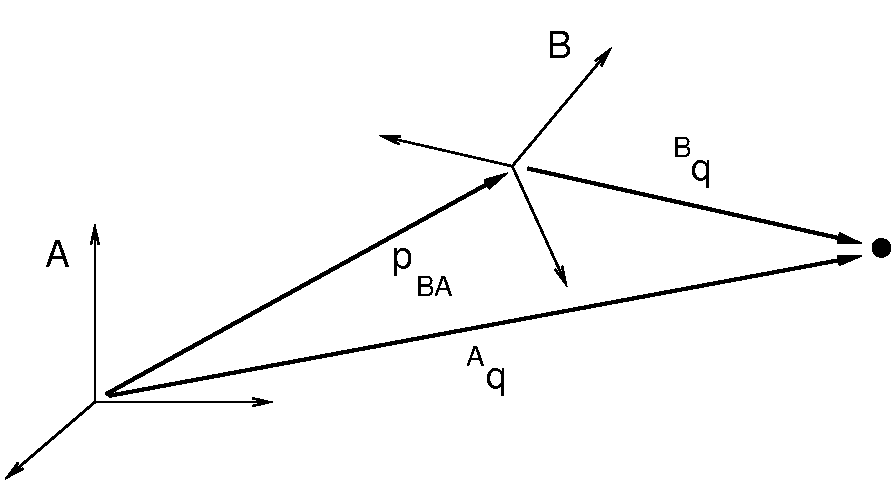
\includegraphics[width=3.75in]{images/pointsAB}
 \else
   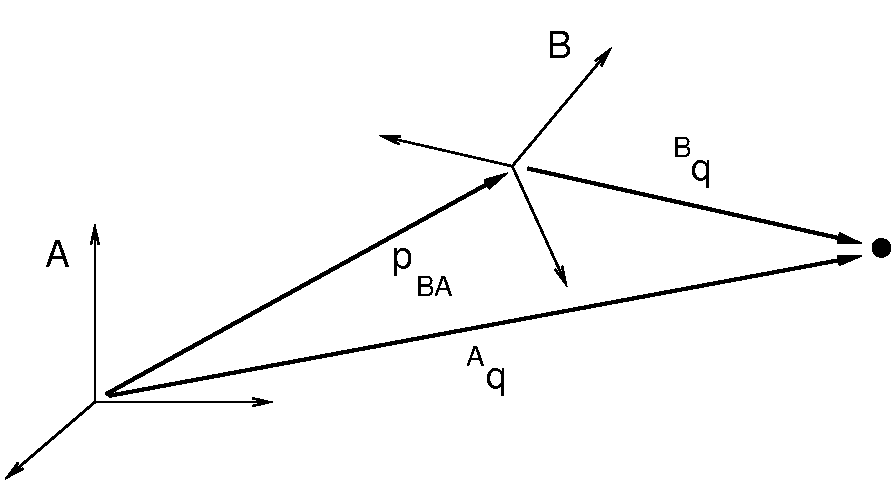
\includegraphics[width=3.75in]{images/pointsAB}
 \fi
\end{center}
\caption{Point vectors ${}^A\q$ and ${}^B\q$ describing
the position of a point $\q$ with respect to frames A and B.}
\label{pointsAB:fig}
\end{figure}

Now, assume we have a 3D point $\q$, and consider its coordinates with
respect to both frames A and B (Figure \ref{pointsAB:fig}). Given the
pose descriptions given above, it is fairly straightforward to show
that
%
\begin{equation}
{}^A\q = \R_{BA} \, {}^B\q + \p_{BA},
\label{pointTransform:eqn}
\end{equation}
%
and, given (\ref{RABinv:eqn}), that
%
\begin{equation}
{}^B\q = \R_{BA}^T \, ({}^A\q - \p_{BA}).
\label{pointInvTransform:eqn}
\end{equation}
%

If we extend our points into a 4D {\it homogeneous} coordinate space
with the fourth coordinate $w$ equal to 1, i.e.,
%
\begin{equation}
\q^* \equiv \matl \q \\ 1 \matr,
\end{equation}
%
then (\ref{pointTransform:eqn}) and
(\ref{pointInvTransform:eqn}) can be simplified to
%
\begin{equation*}
{}^A\q^* = \T_{BA} \, {}^B\q^* \quad \text{and} \quad
{}^B\q^* = \T_{BA}^{-1} \, {}^A\q^*
\end{equation*}
%
where
%
\begin{equation}
\T_{BA} = \matl \R_{BA} & \p_{BA} \\ 0 & 1 \matr
\end{equation}
%
and
%
\begin{equation}
\T_{BA}^{-1} = \matl \R_{BA}^T & -\R_{BA}^T \p_{BA} \\ 0 & 1 \matr.
\end{equation}
%
$\T_{BA}$ is the $4 \times 4$ {\it rigid transform matrix} that
transforms points from B to A and also describes the pose of
B with respect to A (Figure \ref{transformAB:fig}).

\begin{figure}[t]
\begin{center}
 \iflatexml
   \includegraphics[width=3in]{images/transformAB}
 \else
   \includegraphics[width=3in]{images/transformAB}
 \fi
\end{center}
\caption{The transform matrix $\T_{BA}$ from B to A.}
\label{transformAB:fig}
\end{figure}

It is straightforward to show that $\R_{BA}^T$ and $-\R_{BA}^T
\p_{BA}$ describe the orientation and position of $A$ with respect to
$B$, and so therefore
%
\begin{equation}
\T_{BA}^{-1} = \T_{AB}.
\label{transformInverse:eqn}
\end{equation}
%

Note that if we are transforming a vector $\v$ instead of a point
between B and A, then we are only concerned about relative orientation
and the vector transforms (\ref{vectorTransform:eqn}) and
(\ref{vectorInvTransform:eqn}) should be used instead.
However, we can express these using $\T_{BA}$ if
we embed vectors in a homogeneous coordinate space 
with the fourth coordinate $w$ equal to 0, i.e.,
%
\begin{equation}
\v^* \equiv \matl \v \\ 0 \matr,
\end{equation}
%
so that
%
\begin{equation*}
{}^B\v^* = \T_{BA} \, {}^A\v^* \quad \text{and} \quad
{}^A\v^* = \T_{BA}^{-1} \, {}^B\v^*.
\end{equation*}
%

\begin{figure}[t]
\begin{center}
 \iflatexml
   \includegraphics[width=4.5in]{images/transformABC}
 \else
   \includegraphics[width=4.5in]{images/transformABC}
 \fi
\end{center}
\caption{Three coordinate frames A, B, and C and the transforms
relating each one to the other.}
\label{transformsABC:fig}
\end{figure}

Finally, we consider transform composition. Suppose we have three
coordinate frames, A, B, and C, each related to the other by
transforms $\T_{BA}$, $\T_{CB}$, and $\T_{CA}$ (Figure
\ref{transformsABC:fig}).  Using the same reasoning used to derive
(\ref{rotationCB:eqn}) and (\ref{rotationCBII:eqn}), it is easy to
show that
%
\begin{equation}
\T_{CB} = \T_{BA}^{-1} \; \T_{CA} = \T_{AB} \; \T_{CA}.
\end{equation}
%

\section{Affine transforms}
\label{AffineTransforms:sec}

An {\it affine transform} is a generalization of a rigid transform, in
which the rotational component $\R$ is replaced by a general $3 \times
3$ matrix $\A$. This means that an affine transform implements a
generalized basis transformation combined with an offset of the origin
(Figure \ref{affineAB:fig}). As with $\R$ for rigid transforms, the
columns of $\A$ still describe the transformed basis vectors $\x'$,
$\y'$, and $\z'$, but these are generally no longer orthonormal.

\begin{figure}[ht]
\begin{center}
 \iflatexml
    \includegraphics[width=3.25in]{images/affineAB}
 \else
    \includegraphics[width=3.25in]{images/affineAB}
 \fi
\end{center}
\caption{A position vector $\p_{BA}$ and a general matrix $\A_{BA}$
describing the affine position and basis transform of frame B with respect to
frame A.}
\label{affineAB:fig}
\end{figure}

Expressed in terms of homogeneous coordinates,
the affine transform $\X_{AB}$ takes the form
%
\begin{equation}
\X_{BA} = \matl \A_{BA} & \p_{BA} \\ 0 & 1 \matr
\end{equation}
%
with
%
\begin{equation}
\X_{BA}^{-1} = \matl \A_{BA}^{-1} & -\A_{BA}^{-1} \p_{BA} \\ 0 & 1 \matr.
\end{equation}
%
As with rigid transforms, when an affine transform is applied to a
vector instead of a point, only the matrix $\A$ is applied and the
translation component $\p$ is ignored.

Affine transforms are typically used to effect transformations that
require stretching and shearing of a coordinate frame.  By the polar
decomposition theorem, $\A$ can be factored into a regular
rotation $\R$ plus a symmetric shearing/scaling matrix $\P$:
%
\begin{equation}
\A = \R \, \P
\end{equation}
%
Affine transforms can also be used to perform reflections, in which
$\A$ is orthogonal (so that $\A^T \, \A = \I$) but with $\det \A =
-1$.

\section{Rotational velocity}

\begin{figure}[ht]
\begin{center}
 \iflatexml
    \includegraphics[width=3.25in]{images/angularvelAB}
 \else
    \includegraphics[width=3.25in]{images/angularvelAB}
 \fi
\end{center}
\caption{Frame B rotating with respect to frame A.}
\label{angularvelAB:fig}
\end{figure}

Given two 3D coordinate frames A and B, the rotational, or {\it
angular}, velocity of B with respect to A is given by a 3D vector
$\Bom_{BA}$ (Figure \ref{angularvelAB:fig}). $\Bom_{BA}$
is related to the derivative of $\R_{BA}$ by
%
\begin{equation}
\dot\R_{BA} = [{}^A\Bom_{BA}] \R_{BA} = \R_{BA} [{}^B\Bom_{BA}]
\end{equation}
%
where ${}^A\Bom_{BA}$ and ${}^B\Bom_{BA}$ indicate $\Bom_{BA}$ with
respect to frames $A$ and $B$ and $[ \Bom ]$ denotes the $3 \times 3$
cross product matrix
%
\begin{equation}
[ \Bom ] \equiv 
\matl
0 & -\omega_z & \omega_y \\
\omega_z & 0 & -\omega_x \\
-\omega_y & \omega_x & 0 \\
\matr.
\label{xprodmatrix:eqn}
\end{equation}
%

If we consider instead the velocity of $A$ with respect to $B$, it is
straightforward to show that
%
\begin{equation}
\Bom_{AB} = -\Bom_{BA}. 
\end{equation}
%

\section{Spatial velocities and forces}
\label{SpatialVelocitiesAndForces:sec}

Given two 3D coordinate frames A and B, the {\it spatial velocity},
or {\it twist},
$\hat\v_{BA}$ of B with respect to A is given by the 6D 
composition of the translational velocity $\v_{BA}$ of the
origin of B with respect to A and the angular velocity $\Bom_{BA}$:
%
\begin{equation}
\hat\v_{BA} \equiv \matl \v_{BA} \\ \Bom_{BA} \matr.
\end{equation}
%
Similarly, the {\it spatial force}, or {\it wrench}, $\hat\f$ acting
on a frame B is given by the 6D composition of the translational force
$\f_B$ acting on the frame's origin and the moment $\Btau$, or torque,
acting through the frame's origin:
%
\begin{equation}
\hat\f_B \equiv \matl \f_B \\ \Btau_B \matr.
\end{equation}
%

\begin{figure}[ht]
\begin{center}
 \iflatexml
   \includegraphics[width=3.25in]{images/rigidAB}
 \else
   \includegraphics[width=3.25in]{images/rigidAB}
 \fi
\end{center}
\caption{Two frames A and B rigidly connected within a rigid body
and moving with respect to a third frame C.}
\label{rigidAB:fig}
\end{figure}

If we have two frames $A$ and $B$ rigidly connected within a rigid
body (Figure \ref{rigidAB:fig}), and we know the spatial velocity
$\hat\v_{BC}$ of $B$ with respect to some third frame $C$, we may wish
to know the spatial velocity $\hat\v_{AC}$ of $A$ with respect to $C$.
The angular velocity components are the same, but the translational
velocity components are coupled by the angular velocity and the offset
$\p_{BA}$ between $A$ and $B$, so that
%
\begin{equation*}
\v_{AC} = \v_{BC} + \p_{BA} \times \Bom_{BC}.
\end{equation*}
%
$\hat\v_{AC}$ is hence related to $\hat\v_{BC}$ via
\begin{equation*}
\matl \v_{AC} \\ \Bom_{AC} \matr =
\matl \I & [\p_{BA}] \\ 0 & \I \matr \,
\matl \v_{BC} \\ \Bom_{BC} \matr.
\end{equation*}
%
where $[\p_{BA}]$ is defined by
(\ref{xprodmatrix:eqn}).

The above equation assumes that all quantities are expressed
with respect to the same coordinate frame.
If we instead consider $\hat\v_{AC}$ and $\hat\v_{BC}$ to be represented
in frames $A$ and $B$, respectively, then
we can show that
%
\begin{equation}
{}^A\hat\v_{AC} = \X_{BA} \, {}^B\hat\v_{BC},
\end{equation}
%
where
%
\begin{equation}
\X_{BA} \equiv
\matl \R_{BA} & [\p_{BA}] \R_{BA} \\ 0 & \R_{BA} \matr.
\label{XvelAB:eqn}
\end{equation}
%
The transform $\X_{BA}$ is easily formed from the components of the
rigid transform $\T_{BA}$ relating $B$ to $A$.

The spatial forces $\hat\f_A$ and $\hat\f_B$ acting on frames $A$ and
$B$ within a rigid body are related in a similar way, only with
spatial forces, it is the moment that is coupled through the moment
arm created by $\p_{BA}$, so that
%
\begin{equation*}
\Btau_{A} = \Btau_{B} + \p_{BA} \times \f_{B}.
\end{equation*}
%
If we again assume that $\hat\f_A$ and $\hat\f_B$
are expressed in frames $A$ and $B$, we can show that
%
\begin{equation}
{}^A\hat\f_A = \X^*_{BA} \, {}^B\hat\f_B,
\end{equation}
%
where
%
% LaTeXML fails to interpret the [ bracket when directly after \\
\iflatexml
\begin{equation}
\X^*_{BA} \equiv 
\matl \R_{BA} & 0 \\  ~[\p_{BA}]\R_{BA} & \R_{BA} \matr. 
\label{XforceAB:eqn}
\end{equation}
\else
\begin{equation}
\X^*_{BA} \equiv
\matl \R_{BA} & 0 \\  [\p_{BA}] \R_{BA} & \R_{BA} \matr.
\label{XforceAB:eqn}
\end{equation}
\fi


\section{Spatial inertia}
\label{SpatialInertia:sec}

Assume we have a rigid body with mass $m$ and a coordinate frame
located at the body's center of mass.  If $\v$ and $\Bom$ give the
translational and rotational velocity of the coordinate frame, then
the body's linear and angular momentum $\p$ and $\L$ are given by
%
\begin{equation}
\p = m \v \quad \text{and} \quad \L = \J \Bom,
\label{momenta:eqn}
\end{equation}
%
where $\J$ is the $3 \times 3$ {\it rotational inertia} with respect
to the center of mass. These relationships can be combined into a
single equation
%
\begin{equation}
\hat\p = \M \hat\v,
\label{momentum:eqn}
\end{equation}
%
where $\hat\p$ and $\M$ are the {\it spatial momentum} and
{\it spatial inertia}:
%
\begin{equation}
\hat\p \equiv \matl \p \\ \L \matr, \qquad
\M \equiv \matl m \I & 0 \\ 0 & \J \matr.
\end{equation}
%
The spatial momentum satisfies Newton's second law, so that
%
\begin{equation}
\hat\f = \frac{d \hat\p}{dt} = \M \frac{d \hat\v}{dt} + \dot\M \hat\v,
\end{equation}
%
which can be used to find the acceleration of a body in response to a
spatial force.

When the body coordinate frame is {\it not} located at the center of
mass, then the spatial inertia assumes the more complicated form
%
\begin{equation}
\matl 
m \I & -m [\c] \\ m [\c] & \J - m[\c][\c]
\matr,
\end{equation}
%
where $\c$ is the center of mass and $[\c]$ is defined by
(\ref{xprodmatrix:eqn}).

Like the rotational inertia, the spatial inertia is always symmetric
positive definite if $m > 0$.

\ifdefined\maindoc
\else
\end{document}
\fi
